\documentclass[10pt]{exam}

\usepackage[margin=1in]{geometry}
\usepackage{amsmath}
\usepackage{amssymb}
\usepackage{amsthm}
\usepackage{mathtools}
\usepackage{bm}
\usepackage{stmaryrd}

\usepackage{color}
\usepackage{colortbl}
\definecolor{deepblue}{rgb}{0,0,0.5}
\definecolor{deepred}{rgb}{0.6,0,0}
\definecolor{deepgreen}{rgb}{0,0.5,0}
\definecolor{gray}{rgb}{0.7,0.7,0.7}

\usepackage{hyperref}
\hypersetup{
  colorlinks   = true, %Colours links instead of ugly boxes
  urlcolor     = black, %Colour for external hyperlinks
  linkcolor    = blue, %Colour of internal links
  citecolor    = blue  %Colour of citations
}

\usepackage{listings}

%%%%%%%%%%%%%%%%%%%%%%%%%%%%%%%%%%%%%%%%%%%%%%%%%%%%%%%%%%%%%%%%%%%%%%%%%%%%%%%%

\theoremstyle{definition}
\newtheorem{problem}{Problem}
\newtheorem{defn}{Definition}
\newtheorem{refr}{References}
\newtheorem{theorem}{Theorem}
\newcommand{\E}{\mathbb E}
\newcommand{\R}{\mathbb R}
\DeclareMathOperator{\nnz}{nnz}
\DeclareMathOperator{\sign}{sign}
\DeclareMathOperator{\determinant}{det}
\DeclareMathOperator{\Var}{Var}
\DeclareMathOperator{\rank}{rank}
\DeclareMathOperator{\prob}{\mathbb P}
\DeclareMathOperator*{\argmin}{arg\,min}
\DeclareMathOperator*{\argmax}{arg\,max}

\newcommand{\Ein}{E_{\text{in}}}
\newcommand{\Eout}{E_{\text{out}}}
\newcommand{\Etest}{E_{\text{test}}}
\newcommand{\I}{\mathbf I}
\newcommand{\Q}{\mathbf Q}
\newcommand{\p}{\mathbf P}
\newcommand{\pb}{\bar {\p}}
\newcommand{\pbb}{\bar {\pb}}
\newcommand{\pr}{\bm \pi}

\newcommand{\trans}[1]{{#1}^{T}}
\newcommand{\loss}{\ell}
\newcommand{\w}{\mathbf w}
\newcommand{\wstar}{{\w}^{*}}
\newcommand{\x}{\mathbf x}
\newcommand{\y}{\mathbf y}
\newcommand{\lone}[1]{{\lVert {#1} \rVert}_1}
\newcommand{\ltwo}[1]{{\lVert {#1} \rVert}_2}
\newcommand{\lp}[1]{{\lVert {#1} \rVert}_p}
\newcommand{\linf}[1]{{\lVert {#1} \rVert}_\infty}
\newcommand{\lF}[1]{{\lVert {#1} \rVert}_F}

\newcommand{\HH}[1]{\mathcal H_{\text{#1}}}
\newcommand{\Hbinary}{\HH_{\text{binary}}}
\newcommand{\Haxis}{\HH_{\text{axis}}}
\newcommand{\Hperceptron}{\HH_{\text{perceptron}}}


\newcommand{\ignore}[1]{}

%%%%%%%%%%%%%%%%%%%%%%%%%%%%%%%%%%%%%%%%%%%%%%%%%%%%%%%%%%%%%%%%%%%%%%%%%%%%%%%%

\begin{document}


\begin{center}
{
\Huge
%Chapter 1/2: The Learning Problem (III)
Between Chapters 1 and 2
}
\end{center}

\begin{center}
%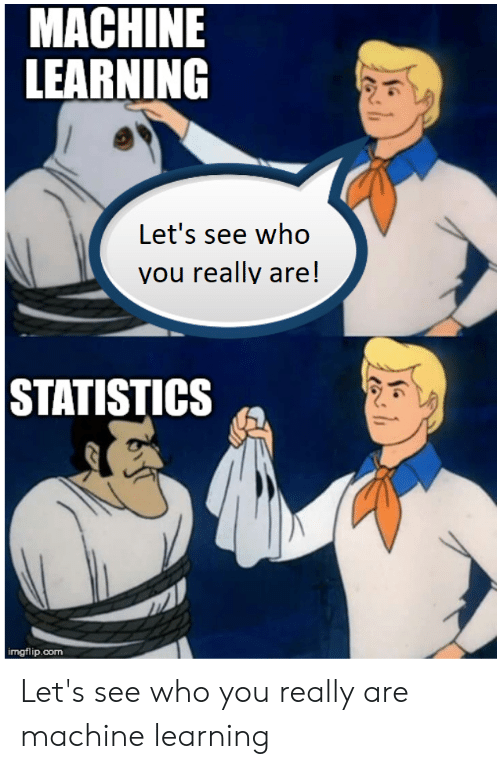
\includegraphics[height=3in]{scooby}
%~~~~~~~~~~
%
\includegraphics[height=3in]{ml}
\end{center}

\noindent
Chapter 2 of the textbook starts discussing the statistical properties of learning algorithms.
Unfortunately, the textbook material jumps in difficulty a LOT between chapters 1 and 2.
The purpose of these notes is to help ``fill the gap.''
In particular, the textbook introduces the idea of \emph{generalization bounds} using infinite hypothesis classes in chapter 2.
Infinite hypothesis classes are fairly abstract and can be a bit tricky to understand;
so we'll start by looking at finite hypothesis classes,
which are more concrete and easier to understand.

%\section{PAC Learning}

%The goal of PAC learning bounds is to help us choose which model to use for a particular problem.
%(Recall that a model is a hypothesis class plus a learning algorithm.)
%In these notes, we will explore some simple, finite hypothesis classes and the simple TEA learning algorithm.

\begin{problem}
    For each hypothesis class below, draw a picture of what a ``typical'' hypothesis looks like and write the number of elements in the hypothesis class.
\begin{align*}
    \HH{binary} &= \bigg\{ \x \mapsto +1, \x \mapsto -1 \bigg\}\\
    \HH{axis} &= \bigg\{ \x \mapsto \sign(x_i) : i \in [d] \bigg\} \\
    \HH{axis2} &= \bigg\{ \x \mapsto \sigma\sign(x_i) : \sigma \in\{+1, -1\}, i \in [d] \bigg\} \\
    \HH{multiaxis2} &= \bigg\{ \x \mapsto \sum_{j=1}^d \sigma_j \sign(x_j) : \sigma_i \in \{+1, -1\}, i \in [d] \bigg\}  \\
    \HH{multiaxis3} &= \bigg\{ \x \mapsto \sum_{j=1}^d \sigma_j \sign(x_j) : \sigma_i \in \{+1, 0, -1\}, i \in [d] \bigg\}  \\
    %\HH{L2-4} &= \bigg\{ \x \mapsto \big\llbracket\ltwo{\x} \ge \alpha \big\rrbracket: \alpha \in \{1, 2, 3, 4\} \bigg\}\\
    %\HH{L1-4} &= \bigg\{ \x \mapsto \big\llbracket \lone{\x} \ge \alpha \big\rrbracket: \alpha \in \{1, 2, 3, 4\} \bigg\}\\
    %\HH{Lp-a} &= \bigg\{ \x \mapsto \big\llbracket \lp{\x} \ge \alpha \big\rrbracket: \alpha \in [a] \bigg\}\\
    %\HH{Lp-a-double} &= \bigg\{ \x \mapsto \sigma\big\llbracket \lp{\x} \ge \alpha \big\rrbracket: \alpha \in [a], \sigma \in \{+1, -1\} \bigg\}\\
\end{align*}
\end{problem}

\newpage
\begin{problem}
    One simple idea for selecting a hypothesis in the hypothesis class is to select the best hypothesis on the training data.
    That is, select
    \begin{equation}
        \label{eq:g}
        g = \argmin_{h\in\mathcal H} \Ein(h)
        .
    \end{equation}
    The \emph{Try Everything Algorithm} (TEA) is a simple algorithm for computing Formula \ref{eq:g} above.
    The pseudo-code is shown below:
    \begin{lstlisting}
    g = None
    g_score = -infinity
    for h in H:
        h_score = E_in(h)
        if h_score > g_score:
            g = h
            g_score = h_score
    \end{lstlisting}
    %What is the runtime of the ERM of the hypothesis classes above?
    What is the runtime of the TEA algorithm?
\end{problem}

\newpage
\noindent
%Equation (2.1) in the textbook states the following theorem.
Page 40 in the textbook defines the following terms and equations.

\begin{defn}
    The \emph{generalization error} of a hypothesis $g$ is defined to be
    $|\Ein(g) - \Eout(g)|$.
\end{defn}

\begin{theorem}[Finite Hypothesis Class Generalization]
    %Equation (1.6) in the textbook states that for any hypothesis class $\mathcal H$ with $M$ entries
    Let $\mathcal H$ be a hypothesis class of size $M$,
    let $g$ be an arbitrary hypothesis in $\mathcal H$
    (in particular, $g$ is allowed to be the result of the TEA algorithm),
    and let $N$ be the size of the dataset.
    Then we have that for all $\epsilon>0$,
    \begin{equation*}
    \prob[|\Ein(g) - \Eout(g)| \ge \epsilon] \le 2M\exp(-2\epsilon^2 N).
    \end{equation*}
    This implies that with probability at least $1-\delta$,
    \begin{equation*}
        \Eout(g) \le \Ein(g) + \sqrt{\frac{1}{2N} \log\frac{2M}{\delta}}.
    \end{equation*}
\end{theorem}
%\begin{proof}
\noindent
    \emph{Proof on pages 23-24 of the textbook.}
%\end{proof}

\vspace{3in}
\begin{problem}
    Graph the in-sample error, out-of-sample error, and the generalization error as a function of the hypothesis class size $M$.

    This should be done informally/at an ``intuition level''; the next two problems explore these trade-offs more formally.
    This is very similar to Figure 2.3 on page 59 of the textbook.
\end{problem}

\newpage
\begin{problem}
    You have a dataset with 100 dimensions and 500 data points.
    Due to the small amount of training data, you have decided not to split the dataset into training and testing datasets,
    and instead you will use the entire dataset for training.
    Your particular application requires that your final model have a generalization error less than 0.1 with probability at least 0.99.
    \begin{enumerate}
        \item
    Which of the finite hypothesis classes above can you select?

            \vspace{4in}
\item
    Of the hypothesis classes that you CAN select, which one SHOULD you select?
    \end{enumerate}

    %You have used the TEA algorithm with the $\HH{multiaxis2}$ hypothesis class on a dataset with 10 dimensions and 10 training points.
\end{problem}

%\begin{theorem}[Union Bound]
    %For any set of events $\mathcal B_1, ..., \mathcal B_n$,
    %we have that
    %\begin{equation}
        %\prob\left(\bigcup_{i=1}^n \mathcal B_i\right)
        %\le
        %\sum_{i=1}^n \prob(\mathcal B_i)
        %.
    %\end{equation}
%\end{theorem}

%\begin{problem}
    %In practice, computers implement IEEE754 floating point arrithmetic rather than real number arithematic.
    %This means that all hypothesis classes (that are used in practice) are actually finite.
%\end{problem}

\newpage
\begin{problem}
    Given two finite hypothesis classes $\HH{1}$ and $\HH{2}$, we can construct a third hypothesis class
    \begin{equation}
        \HH{3} = \HH{1} \cup \HH{2}.
    \end{equation}
    \begin{enumerate}
        \item
            Let $g_i$ be the result of the TEA algorithm on hypothesis class $\HH{i}$.
            How does the in-sample error of $g_3$ compare to the in-sample errors of $g_1$ and $g_2$?
        %How does the training error for $\HH{3}$ compare to the training errors of $\HH{1}$ and $\HH{2}$.

            \vspace{4in}
        \item
            How does the bound on the generalization error from the FHCG theorem for $\HH{3}$ compare to the generalization error of $\HH{1}$ and $\HH{2}$?
    \end{enumerate}
\end{problem}

\end{document}



